% Provenance (never printed): see sources/outline_sources.md (Year 2: climate archives and proxies;
% foraminiferal and ice isotopes; Mg/Ca; pollen; speleothems; tree rings; dating the archives).
% Calibrations after Miller et al. (2020), Groeneveld et al. (2019) and Morley et al. (2024); ice
% cores after White (Geochemistry, ch. 9), Werner et al. (2018) and the EPICA Dome C file of Jouzel
% et al. (2007); age model after Svensson et al. (2008); deep-water context after Wharton et al.
% (2026); figures from figdata/bachelor-2/proxies.py (data/derived lr04, edc-temperature,
% co2-icecore); values of the exercises and problem computed in the Book 4 scratch calculator
% calc/ch24.py.
\chapter{Arsip dan Proksi Iklim}\label{ch:b2:climate-proxies}

Dalam sebuah makalah tahun 1955 seorang ahli geokimia muda melaporkan isotop oksigen cangkang-cangkang mungil
foraminifera yang dipungut dari inti dasar samudra, dan menemukan di dalamnya lima belas siklus glasial--interglasial selama
\num{600000} tahun terakhir. Ia membacanya terutama sebagai suhu: ia hanya mengaitkan sekitar seperlima
ayunan itu dengan es yang tersimpan di daratan. Delapan belas tahun kemudian, Shackleton dan Opdyke menyimpulkan
sebaliknya: efek utamanya adalah penyimpanan air yang ringan secara isotop di dalam lembaran
es. Cangkang yang sama, angka yang sama, dua pembacaan. Cangkang kalsit merekam
suhu air tempat ia tumbuh dan komposisi air itu, dan komposisi
air laut bergantung pada banyaknya es di daratan. Bab ini membahas rekaman-rekaman semacam itu,
arsip yang menyimpannya, proksi yang dibaca darinya, cara proksi itu dikalibrasi terhadap termometer
dan cara penanggalannya, serta seni memisahkan dua sinyal yang dibawa oleh satu cangkang.
% ledger: white13c9:paleo-history

\begin{recall}
\textbf{Dari volume-volume sekolah}: arsip dan \omterm{def:b2:climate-proxies:proxy}{proksi iklim}, inti es, periode glasial dan
interglasial, Maksimum Glasial Terakhir (sekitar \num{23000} sampai \num{19000} tahun yang lalu), analisis
polen. \textbf{Dari volume Tahun 1}: penanggalan radiometrik, umur radiokarbon dan kurva
kalibrasinya; ooze kapur, yang tersusun atas kokolit dan cangkang foraminifera.
\textbf{Dari \cref{ch:b2:isotope-geochemistry}}: \omterm{def:b2:isotope-geochemistry:standards}{standar acuan isotop} \omterm{def:b2:isotope-geochemistry:standards}{VSMOW} dan \omterm{def:b2:isotope-geochemistry:standards}{VPDB}
(\cref{def:b2:isotope-geochemistry:standards}) dan \omterm{prop:b2:isotope-geochemistry:mwl}{garis air meteorik}, $\delta\mathrm{D}
\approx 8\,\delta^{18}\mathrm{O} + 10$ (\cref{prop:b2:isotope-geochemistry:mwl}). \textbf{Dari
buku-buku kimia}: nilai $\delta$ dan faktor fraksionasi. \textbf{Dari buku-buku
matematika}: garis kuadrat terkecil.
\end{recall}
% ledger: ipcc:lgm-cooling, kc98:mwl, kc98:standards

\section{Arsip dan proksi}\label{sec:b2:climate-proxies:archives}

Instrumen baru mengukur iklim belum lama ini. Segala sesuatu yang lebih awal dibaca dari bahan-bahan
yang tumbuh atau mengendap lapis demi lapis sementara iklim bekerja padanya: salju yang berubah menjadi es di
lembaran es kutub, cangkang yang berjatuhan ke dasar samudra, lingkaran tahun pohon, karang, endapan
gua, lumpur danau. Volume-volume sekolah menyebutnya arsip dan besaran yang diukur di dalamnya
proksi; kini kita memerlukan kata-kata yang lebih tajam.

\begin{definition}[Arsip iklim; proksi iklim]\label{def:b2:climate-proxies:proxy}
Yang disebut \emph{arsip iklim}\index{arsip iklim} adalah bahan alami yang terakumulasi
secara bertahap, lapis demi lapis atau lingkaran demi lingkaran, dan mengawetkan ciri-ciri fisis, kimia, atau biologis
lingkungan tempat setiap bagiannya terbentuk. Yang disebut \emph{proksi
iklim}\index{proksi iklim} adalah besaran yang diukur dalam suatu arsip dan bergantung pada suatu variabel
iklim, seperti suhu, jumlah hujan, atau volume es, melalui suatu hubungan yang dapat
dikalibrasi, sehingga menggantikan pengukuran variabel itu yang tidak pernah dilakukan.
\end{definition}
% ledger: ncei:proxy, ncei:paleocean

Tiga sifat menentukan apa yang dapat diceritakan suatu arsip: resolusinya (rentang waktu yang dicakup oleh satu
sampel), jangkauannya (seberapa jauh ke masa lalu) dan cara penanggalannya. Arsip dengan lapisan tahunan dapat
dibaca tahun demi tahun dan ditanggali dengan menghitung; arsip lainnya memerlukan umur radiometrik atau perbandingan dengan
rekaman yang bertanggal. Tabel di bawah membandingkan arsip-arsip dalam bab ini.

\begin{center}
\small
\begin{tabular}{>{\raggedright\arraybackslash}p{0.17\linewidth}>{\raggedright\arraybackslash}p{0.27\linewidth}>{\raggedright\arraybackslash}p{0.21\linewidth}>{\raggedright\arraybackslash}p{0.24\linewidth}}
\hline
arsip & proksi dalam bab ini & lapisan tahunan & penanggalan \\
\hline
sedimen laut dalam & $\delta^{18}$O dan Mg/Ca foraminifera & tidak & radiokarbon, perbandingan dengan
rekaman bertanggal \\
es kutub & $\delta$D dan $\delta^{18}$O es, udara dalam gelembung & di bagian atas inti
yang tebal & menghitung lapisan, lapisan vulkanik bertanggal \\
lingkaran tahun pohon & lebar lingkaran, densitas kayu, isotop & ya & menghitung dan menanggali silang lingkaran \\
\omterm{def:b2:climate-proxies:archives}{speleotem} & $\delta^{18}$O & pada sebagian & penanggalan radiometrik \\
sedimen danau & \omterm{def:b2:climate-proxies:archives}{varve}, polen & bila bervarve & menghitung \omterm{def:b2:climate-proxies:archives}{varve} \\
\hline
\end{tabular}
\end{center}
% ledger: ncei:proxy, ncei:paleocean, ncei:tree-ring, ncei:speleothem, mccarthy23:varves, svensson08:gicc05, noaa:gisp2-layers, bebchuk26:crossdating

Proksi tidak pernah menjadi ukuran murni satu variabel. Lebar lingkaran tahun pohon bergantung pada kehangatan
musim panas dan pada hujan; $\delta^{18}$O cangkang bergantung pada suhu air dan pada
komposisi isotopnya. Pekerjaan ahli paleoklimatologi adalah menemukan proksi yang ketergantungannya
pada variabel yang dicari kuat dan diketahui, mengukur pengaruh-pengaruh lain secara independen, dan
menanggali sampel itu.

\section{Isotop oksigen dalam cangkang karbonat}\label{sec:b2:climate-proxies:oxygen}

Foraminifera adalah protista bersel tunggal, banyak di antaranya membangun cangkang dari kalsit; spesies
planktonik melayang di perairan permukaan, spesies bentik hidup di atas atau di dalam sedimen dasar
laut. Cangkangnya terakumulasi dalam ooze kapur dari volume Tahun 1, dan
$\delta^{18}$O kalsitnya dapat diukur pada beberapa cangkang yang dipungut dari setiap sentimeter suatu
inti.
% ledger: ucmp:forams, ncei:paleocean

\begin{history}[Dua pembacaan atas satu rekaman]
Urey menghitung pada 1947 bagaimana fraksionasi oksigen antara kalsit dan air bergantung pada
suhu, dan mengusulkan bahwa karbonat dapat merekam suhu saat karbonat itu terbentuk. Cesare
Emiliani, yang saat itu muridnya, mengukur $\delta^{18}$O pada foraminifera dari inti piston
samudra-samudra dunia dan menerbitkan pada 1955 sebuah rekaman dengan 15 siklus glasial--interglasial selama
\num{600000} tahun, dengan mengaitkan sekitar \qty{20}{\percent} variasinya dengan volume es.
Pada 1973 Shackleton dan Opdyke menyimpulkan bahwa penyimpanan air yang ringan secara isotop di dalam
lembaran es adalah efek utamanya. Efek vital, yaitu penyimpangan suatu spesies dari kesetimbangan,
dan pertukaran oksigen dengan air pori setelah penimbunan biasanya tidak terlalu penting bagi
cangkang dari beberapa juta tahun terakhir; komposisi isotop air itulah yang penting.
\end{history}
% ledger: white13c9:paleo-history

\subsection*{Suhu}

Kalsit yang tumbuh dalam kesetimbangan dengan air lebih kaya \textsuperscript{18}O daripada air itu,
dan makin dingin airnya, makin besar pengayaannya, seperti yang ditunjukkan perhitungan Urey. Beberapa
kalibrasi empiris menghubungkan
suhu dengan selisih antara $\delta^{18}$O kalsit, pada skala \omterm{def:b2:isotope-geochemistry:standards}{VPDB}, dan
nilai air, pada skala \omterm{def:b2:isotope-geochemistry:standards}{VSMOW}. Untuk laut dalam, satu bentuk yang disederhanakan dipakai bagi cangkang
bentik.

\begin{proposition}[Sebuah kalibrasi bentik]\label{prop:b2:climate-proxies:benthic}
Untuk foraminifera bentik pada suhu laut dalam (di bawah sekitar \qty{13}{\celsius}),
\[
  T = 16.1 - 4.76\,\bigl[\delta^{18}\mathrm{O}_{\mathrm{b}} - (\delta^{18}\mathrm{O}_{\mathrm{sw}} -
  0.27)\bigr],
\]
dengan $T$ dalam \unit{\celsius}, $\delta^{18}\mathrm{O}_{\mathrm{b}}$ nilai cangkang (permil,
\omterm{def:b2:isotope-geochemistry:standards}{VPDB}) dan $\delta^{18}\mathrm{O}_{\mathrm{sw}}$ nilai air laut (permil, \omterm{def:b2:isotope-geochemistry:standards}{VSMOW}); suku
0.27 mengonversi air ke skala kalsit. Pendinginan sebesar \qty{1}{\celsius} pada komposisi air
tetap menaikkan $\delta^{18}\mathrm{O}_{\mathrm{b}}$ sebesar $1/4.76 = 0.21$ permil.
\end{proposition}
\admitted
% ledger: miller20:paleotemp, groeneveld19:anand

Persamaan yang lebih lengkap, yang darinya bentuk itu disederhanakan, memuat suku kuadratik kecil,
$T = 16.1 - 4.64x + 0.09x^2$ dengan $x$ selisih kedua nilai $\delta$; cangkang planktonik
memiliki kalibrasinya sendiri, dengan bentuk yang sama, seperti $T = 14.9 - 4.8\,[\delta^{18}\mathrm{O} -
(\delta^{18}\mathrm{O}_{\mathrm{sw}} - 0.27)]$. Semuanya berbagi satu kesulitan: cangkang memberikan satu
angka, $\delta^{18}\mathrm{O}_{\mathrm{b}}$, sedangkan persamaannya memiliki dua besaran yang tidak diketahui, $T$ dan
$\delta^{18}\mathrm{O}_{\mathrm{sw}}$. Diperlukan proksi kedua yang independen untuk memisahkan keduanya.
% ledger: miller20:paleotemp, groeneveld19:anand

\subsection*{Efek volume es}

Air yang menguap dari laut membawa lebih sedikit \textsuperscript{18}O daripada laut; ketika uap itu
bergerak ke arah kutub dan jatuh sebagai hujan atau salju, uap itu makin terdeplesi, dan salju yang membangun lembaran
es termasuk air paling ringan di planet ini: es Greenland memiliki $\delta^{18}$O sebesar $-30$ sampai $-35$
permil, es Antarktika serendah $-50$. Ketika lembaran es tumbuh, isotop ringan terkunci di daratan
dan samudra yang tertinggal menjadi lebih berat.
% ledger: nasaeo:o18, white:d18o

\begin{definition}[Efek volume es]\label{def:b2:climate-proxies:ice-volume}
Yang disebut \emph{efek volume es}\index{efek volume es} adalah perubahan komposisi isotop oksigen
seluruh samudra yang disebabkan oleh pertumbuhan atau peluruhan lembaran es benua, yang
menyimpan air yang terdeplesi \textsuperscript{18}O; efek ini menggeser $\delta^{18}$O setiap karbonat
yang terbentuk di laut dengan jumlah yang sama, berapa pun suhunya.
\end{definition}
% ledger: nasaeo:o18, white13c9:ice-volume, miller20:paleotemp

\begin{omfigure}
\centering
\begin{tikzpicture}[font=\scriptsize, >=Stealth]
\foreach \col/\title in {0/{a\enspace masa kini}, 7.0/{b\enspace suatu maksimum glasial}} {
  \begin{scope}[shift={(\col,0)}]
  \node[anchor=south west] at (0,3.3) {\textbf{\title}};
  \fill[brown!30] (3.6,0) -- (6.4,0) -- (6.4,1.6) -- (3.6,1.2) -- cycle;
  \end{scope}
}
% today: full ocean, small ice sheet
\fill[ocBlue!25] (0,0) rectangle (3.6,1.2);
\node[align=center] at (1.75,0.55) {samudra\\$\delta^{18}\mathrm{O} = 0$};
\fill[white, draw=black!50] (5.2,1.43) .. controls (5.6,1.95) and (6.2,1.95) .. (6.4,1.6) -- cycle;
\node at (5.0,0.65) {es, $-40$};
\draw[black!50] (5.0,0.85) -- (5.7,1.55);
\draw[->, thick, ocBlue] (1.6,1.35) .. controls (2.4,2.9) and (4.6,2.9) .. (5.6,2.05);
\node at (3.4,3.0) {uap, ringan};
% glacial: lower sea, big ice sheet
\begin{scope}[shift={(7.0,0)}]
\fill[ocBlue!35] (0,0) rectangle (3.6,0.85);
\draw[densely dashed] (0,1.2) -- (3.6,1.2);
\node[anchor=south west, align=left] at (0.05,1.2) {muka laut\\masa kini};
\draw[<->] (3.35,0.85) -- (3.35,1.2);
\node[anchor=east] at (3.3,1.02) {\qty{130}{m}};
\node[align=center] at (1.6,0.42) {samudra, $\delta^{18}\mathrm{O} = +1.46$};
\fill[white, draw=black!50] (3.6,1.2) .. controls (4.0,2.6) and (6.0,2.7) .. (6.4,1.6) -- cycle;
\node at (5.1,1.85) {es, $-40$};
\draw[->, thick, ocBlue] (2.15,0.9) .. controls (2.3,2.6) and (3.3,3.0) .. (4.3,2.6);
\end{scope}
\end{tikzpicture}
\par\smallskip{\small \omterm{def:b2:climate-proxies:ice-volume}{Efek volume es} (skematis, tidak menurut skala): uap yang memasok lembaran
es terdeplesi \textsuperscript{18}O, sehingga menyimpan \qty{130}{m} muka laut sebagai es dengan
$\delta^{18}\mathrm{O} = -40$ permil membuat samudra \num{1.46} permil lebih berat
(\cref{prop:b2:climate-proxies:mass-balance}). Nilai dalam permil, \omterm{def:b2:isotope-geochemistry:standards}{VSMOW}.}
\end{omfigure}
% ledger: nasaeo:o18, miller20:ice-cal, ipcc:lgm-sea

Seberapa besar pergeseran itu? Neraca massa menjawabnya, jika volume es dan komposisi isotop
rata-ratanya diketahui.

\begin{proposition}[Efek volume es dari neraca massa]\label{prop:b2:climate-proxies:mass-balance}
Misalkan samudra masa kini memiliki kedalaman rata-rata $H$ dan $\delta^{18}$O sebesar 0 (\omterm{def:b2:isotope-geochemistry:standards}{VSMOW}). Jika selapis air
laut setebal $h$ diambil dan disimpan di daratan sebagai es dengan komposisi rata-rata
$\delta_{\mathrm{ice}}$, dengan luas samudra dianggap tetap, samudra yang tersisa memiliki
\[
  \Delta\delta^{18}\mathrm{O}_{\mathrm{sw}} = \frac{-h\,\delta_{\mathrm{ice}}}{H - h}.
\]
Untuk $h$ yang kecil, pergeseran itu tumbuh hampir linear, sebesar $-\delta_{\mathrm{ice}}/H$ per meter muka laut.
\end{proposition}

\begin{proof}
Untuk isotop minor, nilai-nilai $\delta$ bergabung seperti konsentrasi: $\delta$ suatu campuran adalah
rata-rata nilai $\delta$ bagian-bagiannya yang dibobot dengan jumlah oksigennya, dan semua
bagian di sini adalah air. Per satuan luas samudra, air samudra masa kini, yaitu kolom $H$ pada
$\delta = 0$, terbagi antara es, $h$ pada $\delta_{\mathrm{ice}}$, dan samudra yang tersisa,
$H - h$ pada $\Delta\delta^{18}\mathrm{O}_{\mathrm{sw}}$:
$H \times 0 = h\,\delta_{\mathrm{ice}} + (H - h)\,\Delta\delta^{18}\mathrm{O}_{\mathrm{sw}}$, yang
memberikan rumus itu. Untuk $h \ll H$, $H - h \approx H$.
\end{proof}
% ledger: white13c9:ice-mass, charette:ocean-volume

\begin{example}[Samudra glasial terakhir]\label{ex:b2:climate-proxies:lgm}
Pada Maksimum Glasial Terakhir muka laut berada 125 sampai \qty{134}{m} di bawah muka laut masa kini; ambil \qty{130}{m},
dengan $H = \qty{3682.2}{m}$, dan es pada $-40$ permil, nilai yang disimpulkan untuk lembaran es besar Amerika
Utara. Maka
$\Delta\delta^{18}\mathrm{O}_{\mathrm{sw}} = 130 \times 40/(3682.2 - 130) = 5200/3552.2 = 1.46$
permil, sekitar $40/3682.2 = 0.0109$ permil per meter muka laut. Perbandingan kurva muka laut
dari teras dan terumbu karang yang bertanggal memberikan \num{0.011} permil per meter, sesuai; skala
\num{0.13} permil per \qty{10}{m}, yang dipakai dalam sebagian rekonstruksi, sesuai dengan es pada sekitar
$-50$ permil. Pengukuran langsung perubahan itu, dari $\delta^{18}$O air yang masih tertahan
di dalam pori sedimen glasial, memberikan $1.0 \pm 0.1$ permil.
\end{example}
% ledger: ipcc:lgm-sea, charette:ocean-volume, miller20:ice-cal, white13c9:ice-volume, wharton26:deep

Gambar di bawah menunjukkan betapa kuatnya jawaban itu bergantung pada komposisi yang diandaikan untuk es.
Selisih antara \num{1.0} dan \num{1.5} permil tidaklah kecil: pada \num{0.21} permil per derajat,
selisih itu setara dengan lebih dari dua derajat suhu samudra dalam. Hubungannya juga tidak sepenuhnya
linear: samudra yang tersisa menyusut ketika es tumbuh, dan $\delta^{18}$O rata-rata es
itu sendiri berubah ketika lembaran-lembaran es dengan komposisi berbeda tumbuh dan meluruh. Rekonstruksi muka laut
dari $\delta^{18}$O karena itu sering memakai hubungan linear yang dikalibrasi pada nilai air pori, sambil
mengakui bahwa hubungan yang sebenarnya seharusnya nonlinear.
% ledger: wharton26:deep, rohling21:linear, miller20:paleotemp

\begin{omfigure}
\centering
% figdata/bachelor-2/proxies.py part icevol
\begin{tikzpicture}
\begin{axis}[width=0.86\linewidth, height=6.0cm, xmin=0, xmax=150, ymin=0, ymax=2.2,
  xlabel={air laut yang tersimpan sebagai es, $h$ (\unit{m} muka laut)},
  ylabel={$\Delta\delta^{18}\mathrm{O}_{\mathrm{sw}}$ (permil)},
  tick label style={font=\scriptsize}, label style={font=\small}, xtick={0,25,...,150},
  legend style={font=\scriptsize, at={(0.5,1.02)}, anchor=south, draw=none, legend columns=4,
  /tikz/every even column/.append style={column sep=6pt}}, legend cell align=left]
\fill[black!10] (axis cs:125,0) rectangle (axis cs:134,2.2);
\addplot[ocBlue, thick] table[x=h_m, y=d30] {figdata/out/bachelor-2-proxies-icevol.dat};
\addlegendentry{es pada $-30$}
\addplot[black, thick] table[x=h_m, y=d40] {figdata/out/bachelor-2-proxies-icevol.dat};
\addlegendentry{es pada $-40$}
\addplot[ocRed, thick] table[x=h_m, y=d50] {figdata/out/bachelor-2-proxies-icevol.dat};
\addlegendentry{es pada $-50$}
\addplot[only marks, mark=square*, mark size=1.8pt, omDef, error bars/.cd, y dir=both,
  y explicit] coordinates {(130,1.0) +- (0,0.1)};
\addlegendentry{air pori}
\addplot[black!60, densely dashed, domain=0:150, samples=2, forget plot] {1.69};
\node[font=\scriptsize, anchor=south west] at (axis cs:3,1.69) {seluruh perubahan LR04, 1.69};
\node[font=\scriptsize, anchor=north, align=center] at (axis cs:112,0.45) {maksimum glasial\\terakhir
$\rightarrow$};
\end{axis}
\end{tikzpicture}
\par\smallskip{\small \omterm{def:b2:climate-proxies:ice-volume}{Efek volume es} dari neraca massa pada
\cref{prop:b2:climate-proxies:mass-balance}, untuk tiga komposisi es (permil, \omterm{def:b2:isotope-geochemistry:standards}{VSMOW});
pita abu-abu: penurunan muka laut Maksimum Glasial Terakhir, 125 sampai \qty{134}{m}; kotak: perubahan
yang diukur dalam air pori sedimen, $1.0 \pm 0.1$ permil, ditempatkan pada \qty{130}{m}; garis putus-putus:
perubahan tumpukan bentik antara masa kini dan Maksimum Glasial Terakhir.}
\end{omfigure}
% ledger: ipcc:lgm-sea, wharton26:deep, data:b4-proxies, miller20:ice-cal

\subsection*{Tumpukan bentik}

Rekaman $\delta^{18}$O bentik dari banyak inti, yang diselaraskan dan dirata-ratakan, membentuk tumpukan (\textit{stack}) yang deraunya
lebih rendah daripada derau inti tunggal mana pun. Tumpukan LR04 menggabungkan 57 rekaman dari situs-situs yang tersebar di
seluruh samudra dunia dan mencakup 5.3 juta tahun. Antara masa kini, \num{3.23} permil, dan rata-rata
\num{19} sampai \qty{23}{ka}, \num{4.92} permil, tumpukan itu berubah sebesar \num{1.69} permil, lebih besar daripada \omterm{def:b2:climate-proxies:ice-volume}{efek volume es}
mana pun yang masuk akal. Seperti yang disimpulkan Shackleton dan Opdyke, sebagian besar perubahan itu adalah es;
tetapi beberapa persepuluh permil tersisa bagi pendinginan air dalam. Soal bab ini mengukur sisa itu.
% ledger: lr04:stack, data:b4-proxies, white13c9:paleo-history, wharton26:deep

\begin{omfigure}
\centering
% figdata/bachelor-2/proxies.py parts lr04, edc, co2
\begin{tikzpicture}
\begin{groupplot}[group style={group size=1 by 3, vertical sep=0.35cm, xlabels at=edge bottom,
  xticklabels at=edge bottom},
  width=0.96\linewidth, height=3.7cm, xmin=0, xmax=800, xtick={0,100,...,800},
  tick label style={font=\scriptsize}, label style={font=\small}]
\nextgroupplot[ylabel={$\delta^{18}\mathrm{O}_{\mathrm{b}}$}, y dir=reverse, ymin=2.45, ymax=5.2,
  ytick={3.5,4.5}]
\addplot[omDef, thin] table[x=age_ka, y=d18O] {figdata/out/bachelor-2-proxies-lr04.dat};
\node[font=\scriptsize, anchor=north east] at (rel axis cs:0.99,0.97) {a\enspace tumpukan LR04 (permil,
VPDB; sumbu dibalik)};
\nextgroupplot[ylabel={$\Delta T$ (\unit{\celsius})}, ymin=-12, ymax=7, ytick={-10,-5,0,5}]
\addplot[ocBlue, thin] table[x=age_ka, y=dT] {figdata/out/bachelor-2-proxies-edc.dat};
\node[font=\scriptsize, anchor=north east] at (rel axis cs:0.99,0.97) {b\enspace anomali suhu
EPICA Dome C};
\nextgroupplot[ylabel={CO$_2$ (\unit{ppm})}, ymin=160, ymax=330, ytick={200,250,300},
  xlabel={umur (ribuan tahun sebelum 1950)}]
\addplot[ocRed, thin] table[x=age_ka, y=co2] {figdata/out/bachelor-2-proxies-co2.dat};
\node[font=\scriptsize, anchor=north east] at (rel axis cs:0.99,0.97) {c\enspace CO$_2$ udara
inti es Antarktika};
\end{groupplot}
\end{tikzpicture}
\par\smallskip{\small \num{800000} tahun terakhir dalam tiga arsip: (a) tumpukan $\delta^{18}$O bentik
LR04, yang diplot dengan sumbu dibalik sehingga masa glasial mengarah ke bawah; (b) anomali
suhu di EPICA Dome C, relatif terhadap rata-rata seribu tahun terakhir, yang diturunkan dari
$\delta$D es; (c) CO$_2$ udara yang terperangkap dalam es Antarktika, sampai 1950. Data: NOAA
NCEI Paleoclimatology (Lisiecki dan Raymo 2005; Jouzel et al.\ 2007; Bereiter et al.\ 2015), sebagaimana
diambil pada 22 Oktober 2026.}
\end{omfigure}
% ledger: data:lr04, data:edc-jouzel, data:co2-bereiter, jouzel07:edc-corr, data:b4-proxies

\section{Inti es}\label{sec:b2:climate-proxies:ice}

Salju yang jatuh di atas lembaran es mempertahankan komposisi isotop yang dimilikinya ketika jatuh, dan
makin dingin tempat dan waktunya, makin ringan salju itu. Di Antarktika suhu udara rata-rata tahunan dan
$\delta^{18}$O salju mengikuti hubungan linear yang kuat dari satu situs ke situs lain, dengan
kemiringan sekitar \num{0.8} permil per derajat, seperti yang diramalkan oleh distilasi Rayleigh uap air dalam perjalanannya
ke pedalaman. Hidrogen dipakai sama seringnya dengan oksigen: pada \omterm{prop:b2:isotope-geochemistry:mwl}{garis air meteorik}, $\delta$D bervariasi sekitar delapan kali lebih cepat daripada $\delta^{18}$O, dan
rekaman $\delta$D es Antarktika dipilih karena kepekaannya yang lebih besar terhadap suhu.
% ledger: werner18:slopes, white13c9:icecore, kc98:mwl

Kemiringan yang diukur menurut ruang belum tentu merupakan kemiringan menurut waktu. Di Greenland, tempat suhu
es itu sendiri telah direkonstruksi dengan metode lain, perubahan $\delta^{18}$O per derajat
menurut waktu ternyata 0.3 sampai \num{0.6} permil, dibandingkan dengan kemiringan spasial masa kini sekitar
\num{0.7}: musim turunnya salju, sumber kelembapan, dan lintasannya berubah bersama
iklim. Suhu-suhu Antarktika yang awal dihitung dengan hubungan spasial yang diukur pada
salju; yang lebih baru memakai model sirkulasi umum yang menyimulasikan isotop air.
% ledger: werner18:slopes, white13c9:icecore

Inti EPICA Dome C, yang dibor menembus \qty{3260}{m} es, mencapai \num{800000} tahun. Nilai
$\delta$D-nya diukur pada sampel sepanjang \qty{55}{cm}, dengan ketelitian \num{0.5} permil, dan
dikonversi menjadi anomali suhu relatif terhadap rata-rata seribu tahun terakhir, setelah
dikoreksi untuk komposisi air laut yang berubah, yang memasok salju itu, dan untuk ketinggian
lembaran es yang berubah. Antara masa glasial dan interglasial suhu bervariasi sekitar
\qty{15}{\celsius}. Antara dua ribu tahun terakhir dan Maksimum Glasial Terakhir (\num{19} sampai
\qty{23}{ka}), $\delta$D rata-rata turun dari $-396.6$ ke $-441.7$ permil dan anomalinya dari
$-0.09$ ke \qty{-9.39}{\celsius}.
% ledger: white13c9:icecore, jouzel07:edc-corr, jouzel07:edc, data:b4-proxies

Es juga menyimpan udara. Firn, yaitu salju padat di puluhan meter teratas, terbuka ke
atmosfer sampai pori-porinya tertutup pada peralihan menjadi es, 50 sampai \qty{120}{m} di bawah permukaan; udara
dalam gelembung karena itu lebih muda daripada es di sekitarnya. Bila diukur dalam gelembung, CO$_2$
udara rata-rata \qty{189.7}{ppm} antara \num{19} dan \qty{23}{ka}, dan \qty{279.4}{ppm} selama
dua ribu tahun sebelum industri. Panel (b) dan (c) pada gambar di atas naik dan turun
bersama selama \num{800000} tahun terakhir.
% ledger: firn:close-off, data:b4-proxies-co2, data:co2-bereiter

Inti Greenland hanya mencapai sekitar \num{120000} tahun, tetapi salju terakumulasi lebih cepat di sana dan
rekamannya lebih halus; rekaman itu menunjukkan penghangatan mendadak pada periode glasial terakhir yang dikenal sebagai
peristiwa Dansgaard--Oeschger. Di dekat puncak inti yang tebal, musim-musim itu sendiri dapat terlihat.
% ledger: white13c9:icecore

\begin{omfigure}
\centering
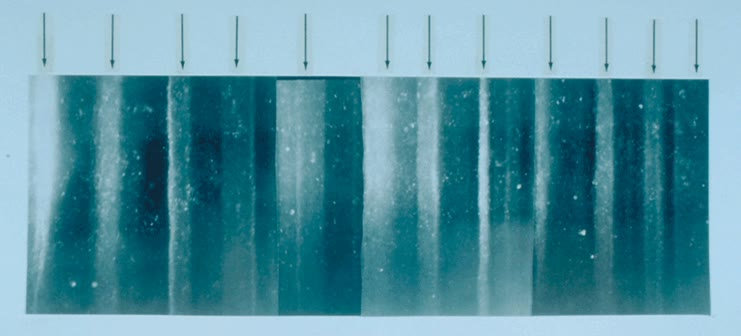
\includegraphics[width=0.72\linewidth]{images/book4/b2-24-gisp2-layers.jpg}
\par\smallskip{\small Sepotong inti es GISP2 dari Greenland tengah pada kedalaman \qty{1855}{m},
yang diterangi dari bawah, dengan lapisan musim panas dan musim dingin yang berselang-seling (panah-panahnya berasal dari
salindia aslinya). Selama musim panas utara yang kering, debu dari Kanada Arktik dan pesisir Greenland
dibawa angin ke atas lembaran es.
(Foto: Anthony Gow, CRREL dari Korps Zeni Angkatan Darat AS, dalam set salindia NOAA Paleoclimatology,
domain publik, via Wikimedia Commons.)}
\end{omfigure}
% ledger: photo:b2-24-gisp2, noaa:gisp2-layers

\begin{inthelab}[Memotong inti es]
\begin{minipage}[t]{0.54\linewidth}\vspace{0pt}
Di sebuah fasilitas inti es nasional, inti-inti disimpan dalam tabung, satu meter inti per tabung, di dalam
pembeku arsip bersuhu \qty{-36}{\celsius}; para ilmuwan bekerja di ruang pemeriksaan bersuhu
\qty{-24}{\celsius}. Ketika inti baru tiba, terbentuklah lini pemrosesan inti: para ilmuwan dan
staf mengukur, mengatalogkan, dan memotong setiap bagian, biasanya 30 sampai \qty{35}{m} sehari, sehingga
inti sepanjang \qty{1000}{m} memerlukan enam sampai delapan pekan. Seorang peneliti menyerut inti itu sampai halus dengan
ketam dan mengukur konduktivitas listriknya, kunci untuk menentukan dan menanggali lapisan-lapisannya; peneliti lain
menggergaji potongan-potongan yang udara terperangkapnya akan dianalisis untuk karbon dioksida dan metana; sampel-sampel itu
lalu dikirim ke laboratorium yang mengukurnya. Di EPICA Dome C, setiap sampel profil $\delta$D
adalah \qty{55}{cm} es.
\end{minipage}\hfill
\begin{minipage}[t]{0.42\linewidth}\vspace{0pt}
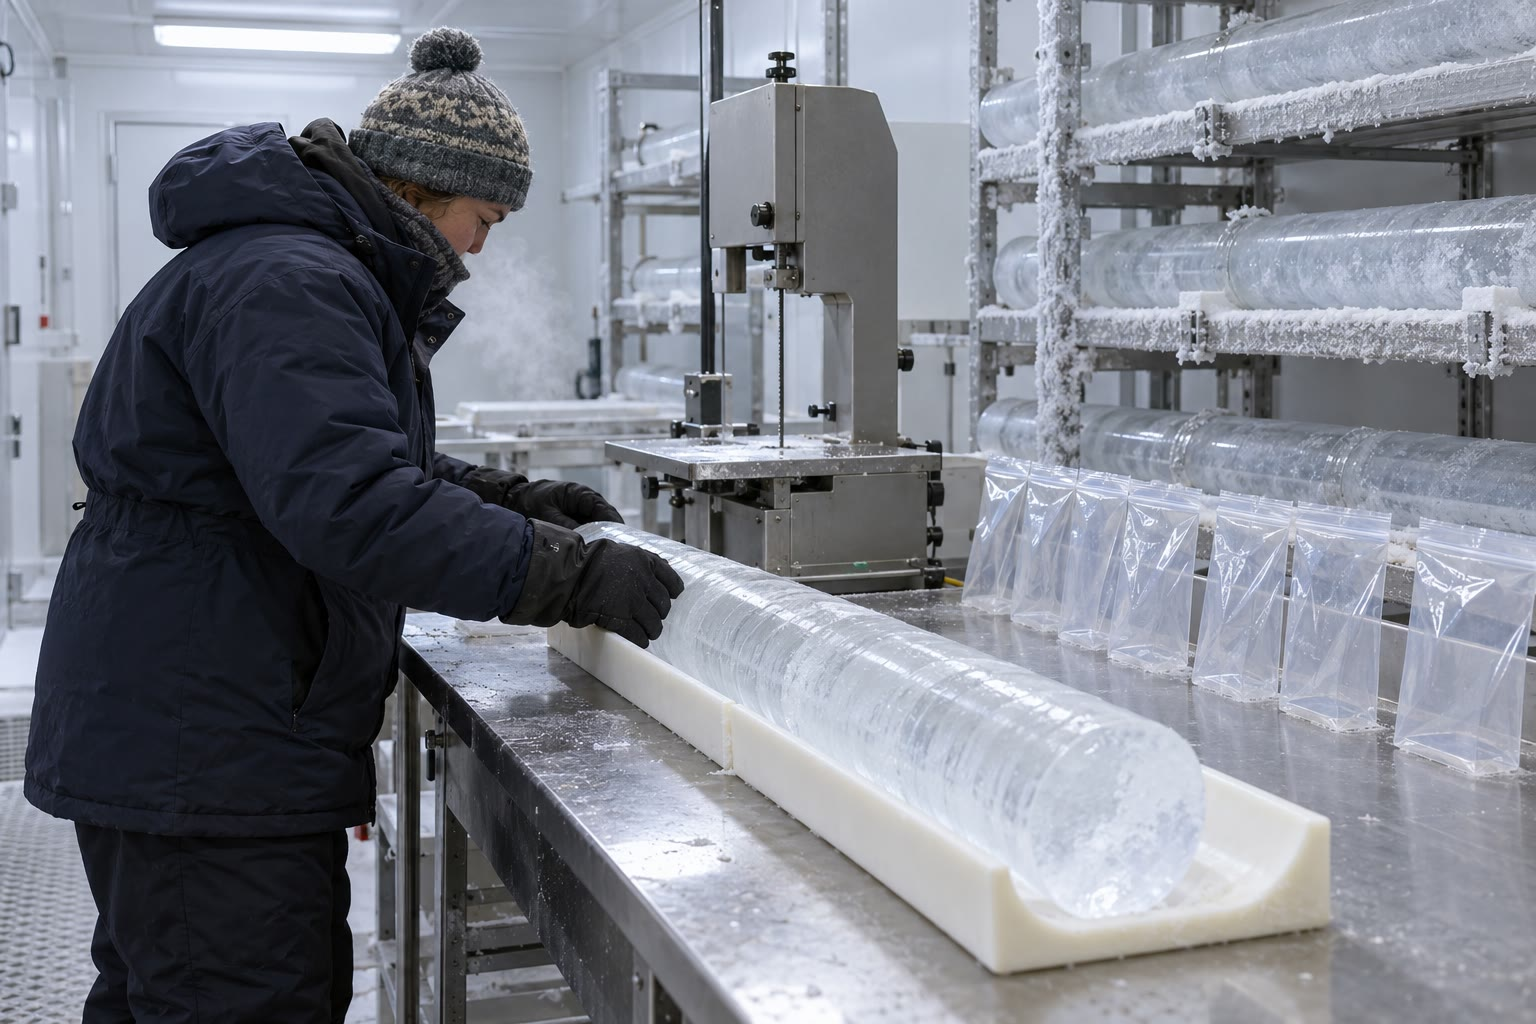
\includegraphics[width=\linewidth]{images/book4/ai/b2-24-cold-lab.jpg}

{\scriptsize Sepotong inti es di atas meja laboratorium dingin, di samping gergaji pita dan kantong
sampel (ilustrasi buatan AI).}
\end{minipage}
\end{inthelab}
% ledger: nsficf:cpl, jouzel07:edc-corr

\section{Proksi lain, arsip lain}\label{sec:b2:climate-proxies:others}

\subsection*{Magnesium dalam cangkang}

Kalsit foraminifera menyerap sedikit magnesium sebagai pengganti kalsium, dan lebih banyak bila
airnya lebih hangat. Rasio itu tidak bergantung pada komposisi isotop air, sehingga
memberikan suhu yang diperlukan oleh persamaan $\delta^{18}$O.

\begin{definition}[Rasio Mg/Ca (proksi)]\label{def:b2:climate-proxies:mgca}
Yang disebut \emph{rasio Mg/Ca (proksi)}\index{rasio Mg/Ca (proksi)} adalah perbandingan magnesium terhadap kalsium dalam
kalsit cangkang foraminifera, dalam \unit{mmol/mol}, yang dipakai sebagai ukuran suhu
air tempat cangkang itu tumbuh melalui kalibrasi eksponensial
\[
  \text{Mg/Ca} = B\,\mathrm{e}^{A T},
\]
dengan $A$ mendekati \qty{0.09}{\per\celsius} untuk spesies planktonik dan $B$ khas untuk setiap spesies.
\end{definition}
% ledger: groeneveld19:anand, morley24:mgca, miller20:paleotemp

Dengan $A = 0.09$ rasio itu tumbuh sebesar $\mathrm{e}^{0.09} - 1 = \qty{9.4}{\percent}$ per derajat,
berapa pun suhunya. Untuk satu spesies planktonik perairan dingin, kalibrasi yang diramalkan dari
suhu saja adalah $\text{Mg/Ca} = 0.4\,\mathrm{e}^{0.09T}$; pencocokan pada 235 cangkang dari jaring
plankton dan puncak inti Atlantik Utara memberikan $0.372\,\mathrm{e}^{0.0936T}$, dengan $r^2 = 0.90$.
Pada suhu rendah rasio yang terukur menyimpang dari kurva itu, dan penyimpangan itu dikaitkan dengan
konsentrasi ion karbonat dalam air laut: suatu proksi jarang bergantung pada satu variabel saja.
Spesies bentik kurang peka, sekitar \qty{0.1}{mmol/mol} per derajat untuk spesies
bermagnesium rendah yang hidup di dalam sedimen.
% ledger: morley24:mgca, wharton26:deep

\begin{omfigure}
\centering
% figdata/bachelor-2/proxies.py part calib
\begin{tikzpicture}
\begin{groupplot}[group style={group size=2 by 1, horizontal sep=1.7cm},
  tick label style={font=\scriptsize}, label style={font=\small}, height=5.2cm,
  width=0.48\linewidth]
\nextgroupplot[xmin=-2, xmax=14, ymin=0, ymax=3.8, xlabel={$T$ (\unit{\celsius})},
  ylabel={$\delta^{18}\mathrm{O}_{\mathrm{b}} - \delta^{18}\mathrm{O}_{\mathrm{sw}}$ (permil)},
  xtick={0,4,...,12}, title={a\enspace $\delta^{18}$O bentik}, title style={font=\scriptsize}]
\addplot[black, thick] table[x=T, y=dd_benthic] {figdata/out/bachelor-2-proxies-calib.dat};
\nextgroupplot[xmin=0, xmax=30, ymin=0, ymax=6.5, xlabel={$T$ (\unit{\celsius})},
  ylabel={Mg/Ca (\unit{mmol/mol})}, xtick={0,5,...,30}, title={b\enspace Mg/Ca planktonik},
  title style={font=\scriptsize},
  legend style={font=\scriptsize, at={(0.03,0.97)}, anchor=north west, draw=none},
  legend cell align=left]
\addplot[ocRed, thick] table[x=T, y=mgca_pred] {figdata/out/bachelor-2-proxies-calib.dat};
\addlegendentry{$0.4\,\mathrm{e}^{0.09T}$}
\addplot[ocBlue, thick, densely dashed] table[x=T, y=mgca_fit]
  {figdata/out/bachelor-2-proxies-calib.dat};
\addlegendentry{$0.372\,\mathrm{e}^{0.0936T}$}
\end{groupplot}
\end{tikzpicture}
\par\smallskip{\small Dua kalibrasi. (a) Kalibrasi bentik pada
\cref{prop:b2:climate-proxies:benthic}: kalsit lebih berat daripada air (pada skalanya
masing-masing) sebesar \num{0.21} permil lebih banyak untuk setiap derajat pendinginan. (b) Mg/Ca suatu spesies
planktonik, sebagaimana diramalkan dari suhu saja dan sebagaimana dicocokkan pada 235 cangkang.}
\end{omfigure}
% ledger: miller20:paleotemp, morley24:mgca

Bila diukur pada cangkang yang sama, Mg/Ca dan $\delta^{18}$O memberikan dua persamaan untuk dua besaran yang tidak diketahui: Mg/Ca
memberikan $T$, lalu \cref{prop:b2:climate-proxies:benthic} memberikan
$\delta^{18}\mathrm{O}_{\mathrm{sw}}$, yaitu sinyal volume es. Bila diterapkan pada cangkang bentik dari laut dalam
Atlantik Barat Laut, metode itu mendapati air Maksimum Glasial Terakhir hanya sekitar
\qty{2}{\celsius} lebih dingin daripada air masa kini ($-1.78 \pm \qty{0.56}{\celsius}$), sedangkan perkiraan dari
air pori menempatkan kedua massa air dalam dekat titik beku di samudra glasial, $-1.1$ dan
\qty{-1.9}{\celsius}, padahal kini keduanya bersuhu 2 sampai \qty{4}{\celsius} dan 0 sampai \qty{1}{\celsius}.
% ledger: miller20:paleotemp, wharton26:deep

\subsection*{Lingkaran tahun pohon}

\begin{definition}[Dendroklimatologi; penanggalan silang]\label{def:b2:climate-proxies:dendro}
Yang disebut \emph{dendroklimatologi}\index{dendroklimatologi} adalah rekonstruksi iklim masa lalu dari
lingkaran pertumbuhan tahunan pohon: lebarnya, densitas kayunya, dan komposisi
isotopnya. Yang disebut \emph{penanggalan silang}\index{penanggalan silang} adalah pencocokan pola lingkaran lebar dan
sempit antarpohon, yang menetapkan tahun kalender mutlak setiap lingkaran dan mengungkap
lingkaran yang secara lokal tidak ada pada satu pohon.
\end{definition}
% ledger: bebchuk26:crossdating, bebchuk26:absent-rings, ncei:tree-ring, ncei:proxy

Lingkaran lebih lebar bila kondisi mendukung pertumbuhan. \omterm{def:b2:climate-proxies:dendro}{Penanggalan silang} andal di situs yang iklimnya ekstrem, tempat satu
faktor iklim membatasi pertumbuhan semua pohon, sehingga pohon-pohon itu berbagi pola yang sama; \omterm{def:b2:climate-proxies:dendro}{penanggalan silang} dapat
gagal bila tidak ada satu faktor pun yang dominan, dan bila banyak lingkaran yang secara lokal tidak ada.
Menumpangtindihkan pola pohon hidup, kayu bangunan tua, dan kayu terkubur memperpanjang kronologi ke masa lalu
tahun demi tahun; sebuah studi baru-baru ini menanggali kronologi 100 pohon yew subfosil dari Inggris timur pada
456 tahun dari 2668 sampai 2213 SM, dengan memakai $\delta^{18}$O lebih dari \num{1500} lingkarannya
terhadap kronologi pohon ek yang bertanggal mutlak. International Tree-Ring Data Bank menyimpan lebar
lingkaran, densitas, isotop, dan kronologi dari lebih dari \num{5000} situs di enam benua.
% ledger: ncei:proxy, bebchuk26:crossdating, bebchuk26:absent-rings, ncei:tree-ring

\subsection*{Gua dan danau}

\begin{definition}[Speleotem; varve]\label{def:b2:climate-proxies:archives}
Yang disebut \emph{speleotem}\index{speleotem} adalah endapan mineral yang terbentuk dari air tanah di dalam
gua: stalagmit, stalaktit, dan bentuk-bentuk lain. Yang disebut \emph{varve}\index{varve} adalah
endapan satu tahun dalam sedimen dasar danau atau laut, biasanya sepasang lamina dengan
komposisi yang kontras, satu diendapkan pada musim panas dan satu lagi pada sisa tahun itu.
\end{definition}
% ledger: ncei:speleothem, mccarthy23:varves

\omterm{def:b2:climate-proxies:archives}{Speleotem} tumbuh lapis demi lapis dari air tanah yang mencapai gua; ketebalan
lapisan-lapisannya dan rekaman isotopnya memberikan kondisi iklim masa lalu. Sebagian memiliki pita tahunan,
dan sebagian mengandung senyawa yang dapat ditanggali secara radiometrik. Skala waktu inti Greenland sesuai dengan skala waktu
\omterm{def:b2:climate-proxies:archives}{speleotem} Gua Hulu sampai dalam 800 tahun selama \num{60000} tahun terakhir: dua
arsip, yang ditanggali dengan metode berbeda, saling memeriksa.
% ledger: ncei:speleothem, svensson08:gicc05

\begin{omfigure}
\centering
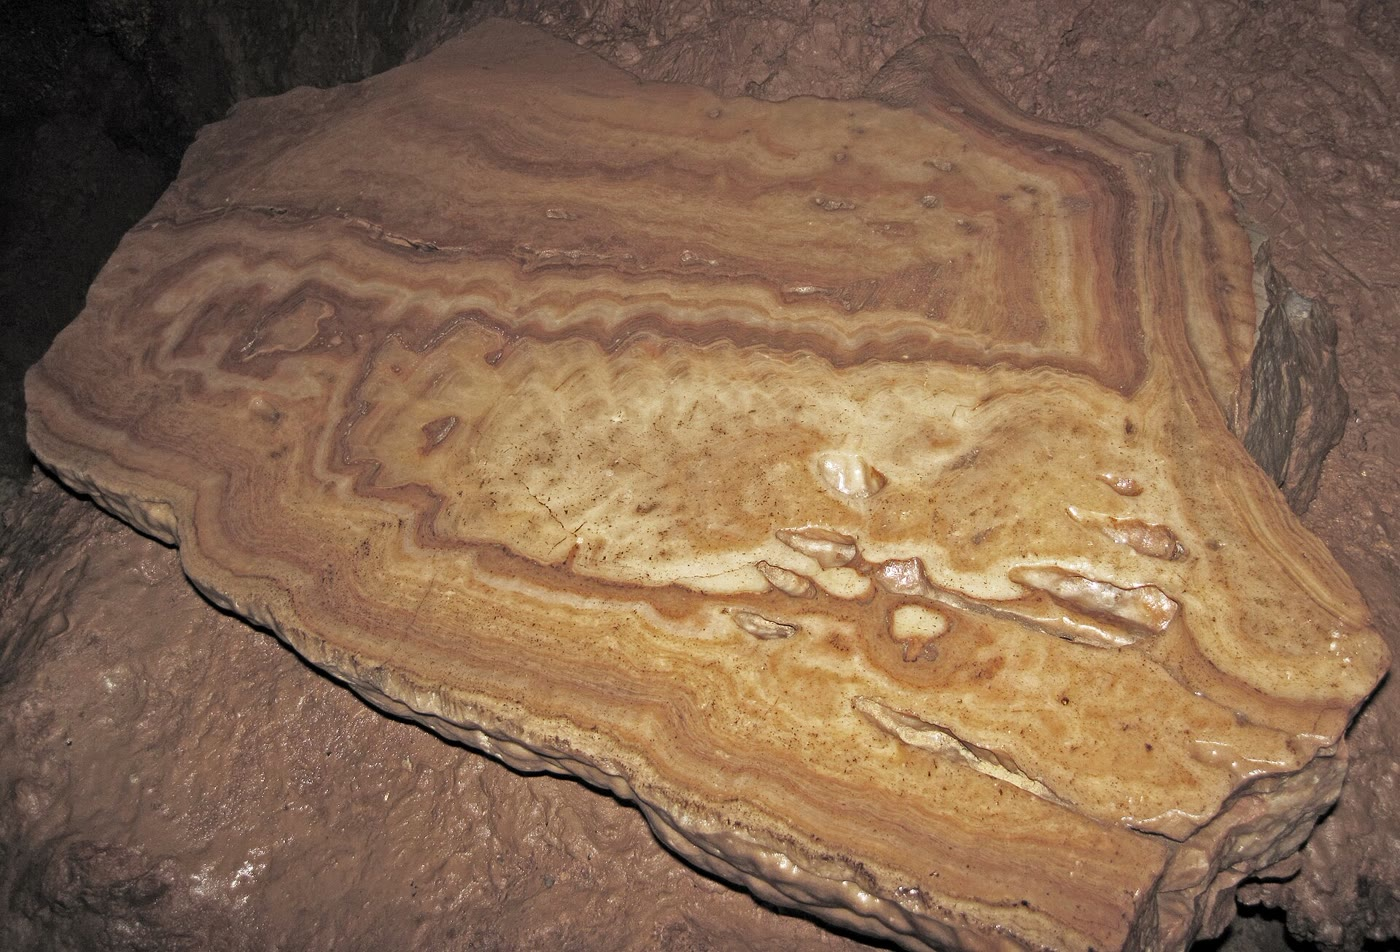
\includegraphics[width=0.62\linewidth]{images/book4/b2-24-speleothem.jpg}
\par\smallskip{\small Penampang \omterm{def:b2:climate-proxies:archives}{speleotem} kalsit yang dipotong dan dipoles dari Diamond Caverns,
Kentucky, yang diwarnai oleh pengotor oksida besi: setiap pita dulunya adalah permukaan endapan itu.
(Foto: James St.~John, CC BY 2.0, via Wikimedia Commons.)}
\end{omfigure}
% ledger: photo:b2-24-speleothem

Di cekungan dalam Danau Crawford, di Ontario, air dasarnya, yang lebih asin dan lebih basa daripada
air di atasnya, tidak memuat hewan yang cukup besar untuk mengaduk lumpur, meskipun airnya kaya
oksigen, dan setiap tahun menambahkan sepasang lapisan: lapisan bahan organik, yang ditutup oleh
kalsit yang mengendap setiap musim panas dari air permukaan yang basa. Sedimen danau juga menyimpan
polen vegetasi di sekitarnya, yang dibaca dengan analisis polen; bervarve atau tidak, sedimen itu merekam
daratan.
% ledger: mccarthy23:varves, mccarthy23:no-bioturbation, ncei:pollen

\section{Model umur}\label{sec:b2:climate-proxies:age}

Proksi tanpa tanggal hanyalah keanehan. Setiap arsip memerlukan hubungan antara kedalaman, atau lingkaran, atau
pita, dan umur.

\begin{definition}[Model umur; penghitungan lapisan tahunan]\label{def:b2:climate-proxies:age-model}
Yang disebut \emph{model umur}\index{model umur} adalah fungsi yang menetapkan umur, beserta ketidakpastiannya, bagi
setiap kedalaman suatu arsip. Yang disebut \emph{penghitungan lapisan tahunan}\index{penghitungan lapisan tahunan} membangun model
umur dengan menghitung, dari atas ke bawah, lapisan-lapisan yang masing-masing merekam satu tahun (lapisan es, \omterm{def:b2:climate-proxies:archives}{varve},
pita), dengan setiap lapisan yang sifat tahunannya diragukan dihitung sebagai setengah tahun plus minus
setengah tahun.
\end{definition}
% ledger: svensson08:gicc05, mccarthy23:varves

\begin{method}[Membangun model umur]\label{met:b2:climate-proxies:age-model}
\begin{enumerate}
  \item Bila arsip memiliki lapisan tahunan, hitunglah lapisan-lapisan itu dari puncak yang diketahui, dengan mencatat lapisan yang tidak pasti
        secara terpisah.
  \item Bila arsip tidak memilikinya, atau lapisan itu tidak dapat dibedakan, tetapkan \emph{titik ikat}: kedalaman yang ditanggali
        secara independen, dengan radiokarbon atau metode radiometrik lain, dengan abu vulkanik yang bertanggal, atau dengan
        mencocokkannya dengan rekaman yang bertanggal baik.
  \item Di antara titik-titik ikat, lakukan interpolasi, linear terhadap kedalaman jika tidak ada yang lebih baik, atau dengan
        model tentang cara arsip itu terakumulasi dan menipis.
  \item Bawalah ketidakpastian setiap langkah ke setiap kedalaman.
\end{enumerate}
\end{method}
% ledger: svensson08:gicc05, noaa:gisp2-layers, ncei:speleothem

Kronologi Inti Es Greenland 2005, GICC05, menghitung lapisan tahunan dalam tiga inti Greenland, dan
pada bagian glasial dalam inti NorthGRIP saja, selama \num{60000} tahun terakhir; umurnya
dinyatakan dalam tahun sebelum 2000 M, ditulis b2k. Lapisan yang tidak pasti, yang dihitung sebagai $\frac12 \pm \frac12$,
dijumlahkan menjadi \emph{galat hitung maksimum}, yang dianggap para penulisnya sebagai dua simpangan baku.
Pada awal Holosen, 11\,703 tahun b2k, galat itu 50 tahun; pada awal
interstadial Greenland 17, \num{59440} tahun b2k, galat itu \num{1287} tahun.
% ledger: svensson08:gicc05, svensson08:table1

\begin{proposition}[Pertumbuhan galat hitung]\label{prop:b2:climate-proxies:counting}
Misalkan suatu hitungan memuat $n$ lapisan yang tidak pasti, masing-masing dihitung sebagai $\frac12$ dengan galat bersimpangan
baku $\frac12$. Jika galat lapisan-lapisan itu independen, simpangan baku
totalnya $\frac12\sqrt{n}$; jika semuanya bertanda sama, galat totalnya
$\frac12 n$.
\end{proposition}

\begin{proof}
Varians jumlah galat yang independen adalah jumlah variansnya: $n \times
(\frac12)^2$, yang akar kuadratnya $\frac12\sqrt{n}$. Jika setiap lapisan keliru ke arah yang sama,
galat-galat itu dijumlahkan sebagai bilangan biasa: $n \times \frac12$.
\end{proof}

Pada GI-17, galat hitung maksimum sebesar \num{1287} tahun berarti \num{2574} lapisan yang tidak pasti. Seandainya
galat-galatnya independen, totalnya hanya akan tidak pasti sebesar $\frac12\sqrt{2574} = 25$ tahun.
Jumlah linear adalah pilihan yang hati-hati: lapisan-lapisan yang meragukan pada satu bentang es dinilai oleh
penghitung yang sama dengan kriteria yang sama, dan tidak ada alasan untuk mengharapkan galat-galatnya saling meniadakan.
Bagian rekaman yang lebih tua dihitung secara independen oleh dua orang penulisnya; hitungan mereka
berbeda kurang dari galat mutlaknya, meskipun secara lokal lebih dari galat hitung akhirnya. Galat
hitung maksimum rata-rata sekitar \qty{1}{\percent} dari waktu yang dicakup suatu bagian pada Holosen dan
\qty{5}{\percent} pada bagian glasial.
% ledger: svensson08:gicc05, svensson08:table1, svensson08:two-counters

\begin{omfigure}
\centering
% figdata/bachelor-2/proxies.py part gicc05
\begin{tikzpicture}
\begin{groupplot}[group style={group size=2 by 1, horizontal sep=1.7cm},
  tick label style={font=\scriptsize}, label style={font=\small}, height=5.4cm,
  width=0.48\linewidth, xmin=0, xmax=62, xlabel={umur GICC05 (\unit{ka} b2k)}]
\nextgroupplot[ymin=1450, ymax=2450, y dir=reverse, ylabel={kedalaman NorthGRIP (\unit{m})},
  title={a\enspace kedalaman dan umur}, title style={font=\scriptsize}]
\addplot[black, mark=*, mark size=1.1pt] table[x=age_ka, y=depth_m]
  {figdata/out/bachelor-2-proxies-gicc05.dat};
\nextgroupplot[ymode=log, ymin=2, ymax=30000, ylabel={ketidakpastian (tahun)},
  title={b\enspace ketidakpastian hitungan}, title style={font=\scriptsize},
  legend style={font=\scriptsize, at={(0.03,0.97)}, anchor=north west, draw=none},
  legend cell align=left]
\addplot[ocRed, mark=*, mark size=1.1pt] table[x=age_ka, y=err_yr]
  {figdata/out/bachelor-2-proxies-gicc05.dat};
\addlegendentry{galat hitung maksimum}
\addplot[ocBlue, mark=o, mark size=1.1pt] table[x=age_ka, y=err_random_yr]
  {figdata/out/bachelor-2-proxies-gicc05.dat};
\addlegendentry{jika independen}
\end{groupplot}
\end{tikzpicture}
\par\smallskip{\small Kronologi GICC05 pada 18 peristiwa iklim dari awal Holosen sampai
\qty{59.44}{ka}: (a) kedalaman dalam inti NorthGRIP terhadap umur; kurvanya melandai ketika lapisan tahunan
menipis seiring kedalaman, sehingga setiap seribu tahun menempati lebih sedikit meter es; (b) galat hitung maksimum, dan galat yang akan diberikan oleh jumlah lapisan
tidak pasti yang sama jika galat-galatnya independen (\cref{prop:b2:climate-proxies:counting});
skala logaritmik. Data: Svensson et al.\ (2008), Tabel 1.}
\end{omfigure}
% ledger: svensson08:table1, svensson08:gicc05

Lapisan tahunan menipis seiring kedalaman, karena es mengalir dan menyebar ketika tenggelam: antara awal
Holosen dan GI-1, lapisan rata-rata setebal \qty{3.75}{cm} di NorthGRIP; antara GI-16 dan
GI-17, \qty{1.54}{cm}; sekitar \qty{100}{ka}, model aliran menempatkannya dekat \qty{1}{cm}. Makin tipis lapisan, makin sukar
lapisan-lapisan itu dibedakan.
% ledger: svensson08:table1, svensson08:gicc05

\section{Kalibrasi}\label{sec:b2:climate-proxies:calibration}

Setiap angka yang dibaca dari suatu proksi datang melalui suatu kalibrasi.

\begin{definition}[Kalibrasi proksi]\label{def:b2:climate-proxies:calibration}
Yang disebut \emph{kalibrasi proksi}\index{kalibrasi proksi} adalah hubungan empiris atau teoretis yang
mengonversi nilai suatu proksi menjadi variabel iklim yang diwakilinya, yang ditetapkan pada sampel-sampel yang
kedua nilainya diketahui, beserta ketidakpastiannya dan rentang kondisi tempat hubungan itu
berlaku.
\end{definition}
% ledger: morley24:mgca, miller20:paleotemp

Sampel yang kedua nilainya diketahui adalah sampel modern: cangkang yang ditangkap dengan jaring plankton, puncak inti sedimen yang dibandingkan dengan air di atasnya, salju baru yang dibandingkan dengan
suhu situsnya, lingkaran terluar pohon yang dibandingkan dengan catatan stasiun cuaca.
Hubungan itu lalu dicocokkan dengan kuadrat terkecil; untuk hukum eksponensial seperti kalibrasi
Mg/Ca, pencocokan dilakukan pada logaritmanya, yang mengubah $\text{Mg/Ca} = B\,\mathrm{e}^{AT}$ menjadi
garis lurus $\ln(\text{Mg/Ca}) = \ln B + AT$. Suatu kalibrasi divalidasi pada sampel-sampel yang
tidak dipakai untuk mencocokkannya: sebagian data modern disisihkan dan diramalkan.
% ledger: morley24:mgca, werner18:slopes, ncei:tree-ring

Tiga batasan tetap ada. Kalibrasi yang diukur menurut ruang, dari tempat ke tempat pada masa kini, mungkin tidak berlaku
menurut waktu, seperti yang telah ditunjukkan es Greenland. Kalibrasi yang diukur pada rentang kondisi masa kini
harus diekstrapolasi dengan hati-hati: Mg/Ca cangkang menyimpang dari hukumnya pada suhu rendah, tempat
variabel lain, yaitu ion karbonat, mengambil alih. Dan hubungan yang linear pada rentang kecil
mungkin tidak linear pada rentang besar, seperti \omterm{def:b2:climate-proxies:ice-volume}{efek volume es}. Metode bab ini
menjawab ketiganya dengan cara yang sama: ukurlah dua proksi independen pada sampel yang sama, dan biarkan masing-masing
memeriksa yang lain.
% ledger: werner18:slopes, morley24:mgca, rohling21:linear

\section*{Latihan}\label{sec:b2:climate-proxies:exercises}

Data untuk latihan, kecuali dinyatakan lain: kedalaman samudra rata-rata $H = \qty{3682.2}{m}$, luas
samudra \qty{361.84e6}{km^2}; kalibrasi bentik pada \cref{prop:b2:climate-proxies:benthic}; kalibrasi
planktonik $\text{Mg/Ca} = 0.4\,\mathrm{e}^{0.09T}$ (\unit{mmol/mol}, \unit{\celsius});
nilai $\delta$ air dan es dalam permil \omterm{def:b2:isotope-geochemistry:standards}{VSMOW}, nilai kalsit dalam permil \omterm{def:b2:isotope-geochemistry:standards}{VPDB}.
% ledger: charette:ocean-volume, miller20:paleotemp, morley24:mgca

\begin{exercise}[$\star$]\label{exo:b2:climate-proxies:1}
Kini es benua menyimpan sekitar \qty{27.5e6}{km^3} dan samudra \qty{1350e6}{km^3}
air (anggaplah volume itu sebagai jumlah air). (a) Jika es memiliki $\delta^{18}$O rata-rata $-30$
permil dan samudra 0, berapa $\delta^{18}$O seluruh hidrosfer, dengan mengabaikan air
tawar? (b) Jika seluruh es mencair, menjadi berapa $\delta^{18}$O samudra? (c) Berapa
bagian air yang berupa es?
\end{exercise}
% ledger: white13c9:ice-mass

\begin{exercise}[$\star$]\label{exo:b2:climate-proxies:2}
Sebuah cangkang bentik memiliki $\delta^{18}\mathrm{O}_{\mathrm{b}} = 2.50$ permil. (a) Hitung
suhunya jika air laut memiliki $\delta^{18}\mathrm{O}_{\mathrm{sw}} = 0$. (b) Hitung suhunya jika
air laut memiliki $+1.0$ permil. (c) Cangkang lain, dari air yang sama pada $0$ permil, memiliki
$2.71$ permil: seberapa lebih dingin airnya?
\end{exercise}
% ledger: miller20:paleotemp

\begin{exercise}[$\star$]\label{exo:b2:climate-proxies:3}
(a) Hitung rasio Mg/Ca menurut kalibrasi planktonik pada \qty{10}{\celsius} dan pada
\qty{20}{\celsius}. (b) Dengan faktor berapa rasio itu tumbuh selama sepuluh derajat ini, dan berapa
persen per derajat? (c) Hitung suhu cangkang dengan Mg/Ca = 2.0 dan
\qty{1.0}{mmol/mol}.
\end{exercise}
% ledger: morley24:mgca

\begin{exercise}[$\star$]\label{exo:b2:climate-proxies:4}
Sebuah kronologi pohon yew subfosil berlangsung dari 2668 sampai 2213 SM. (a) Berapa tahun yang dicakupnya,
dengan menghitung kedua tahun ujungnya? (b) Mengapa kronologi yang dibangun dari banyak pohon lebih layak dipercaya daripada
hitungan lingkaran satu pohon saja? (c) Mengapa kamu dapat mengharapkan \omterm{def:b2:climate-proxies:dendro}{penanggalan silang} lebih mudah bagi
pohon di dekat batas pohon yang dingin daripada bagi pohon di hutan dataran rendah yang beriklim lunak dan lembap?
\end{exercise}
% ledger: bebchuk26:crossdating

\begin{exercise}[$\star\star$]\label{exo:b2:climate-proxies:5}
(a) Dengan \cref{prop:b2:climate-proxies:mass-balance}, hitung \omterm{def:b2:climate-proxies:ice-volume}{efek volume es} untuk penurunan muka laut
sebesar \qty{125}{m} dan \qty{134}{m}, dengan es pada $-40$ permil. (b) Hitung efek itu untuk
\qty{130}{m} dengan es pada $-30$, $-35$, dan $-50$ permil. (c) Komposisi es rata-rata mana
yang akan membuat efek penurunan \qty{130}{m} sama dengan \num{1.0} permil yang diukur dalam air
pori? Bandingkan dengan komposisi lembaran es masa kini.
\end{exercise}
% ledger: ipcc:lgm-sea, white:d18o, miller20:ice-cal, wharton26:deep

\begin{exercise}[$\star\star$]\label{exo:b2:climate-proxies:6}
Bandingkan kedua kalibrasi Mg/Ca untuk spesies planktonik yang sama: kalibrasi yang diramalkan dari
suhu saja, $0.4\,\mathrm{e}^{0.09T}$, dan hasil pencocokan $0.372\,\mathrm{e}^{0.0936T}$. (a) Pada
suhu berapa keduanya sama? (b) Pada \qty{2}{\celsius}, berapa persen rasio hasil pencocokan
lebih rendah daripada rasio yang diramalkan? (c) Sebuah cangkang yang tumbuh pada \qty{2}{\celsius} mengikuti hukum hasil pencocokan; suhu
berapa yang akan diberikan hukum ramalan untuknya?
\end{exercise}
% ledger: morley24:mgca

\begin{exercise}[$\star\star$]\label{exo:b2:climate-proxies:7}
Dalam inti NorthGRIP, awal Holosen terletak pada \qty{1492.45}{m} dan \num{11703} tahun
b2k, awal GI-1 pada \qty{1604.64}{m} dan \num{14692} tahun; awal GI-16 pada
\qty{2402.55}{m} dan \num{58280} tahun, awal GI-17 pada \qty{2420.44}{m} dan \num{59440} tahun.
(a) Hitung ketebalan rata-rata lapisan tahunan pada setiap selang. (b) Mengapa lapisan-lapisan itu lebih tipis
di bagian yang lebih dalam? (c) Mengapa \omterm{def:b2:climate-proxies:age-model}{penghitungan lapisan tahunan} menjadi mustahil pada kedalaman tertentu?
\end{exercise}
% ledger: svensson08:table1, svensson08:gicc05

\begin{exercise}[$\star\star$]\label{exo:b2:climate-proxies:8}
Gunakan dua titik ikat pertama dari \cref{exo:b2:climate-proxies:7}, dengan galat hitung maksimum 50
dan 93 tahun. (a) Dengan interpolasi linear terhadap kedalaman, berikan umur es pada \qty{1550}{m}.
(b) Nyatakan umur itu dalam tahun sebelum 1950. (c) Interpolasikan ketidakpastiannya dengan cara yang sama.
\end{exercise}
% ledger: svensson08:table1

\begin{exercise}[$\star\star$]\label{exo:b2:climate-proxies:9}
Galat hitung maksimum GICC05 adalah 93 tahun pada GI-1 dan \num{1287} tahun pada GI-17. (a) Berapa banyak
lapisan tidak pasti yang diwakili masing-masing? (b) Berapa ketidakpastiannya jika galat lapisan-lapisan
itu independen, masing-masing dengan simpangan baku setengah tahun? (c) Dengan faktor berapa
jumlah linear melampaui perkiraan independen pada setiap kasus, dan mengapa faktor itu tumbuh seiring kedalaman?
\end{exercise}
% ledger: svensson08:gicc05, svensson08:table1

\begin{exercise}[$\star\star\star$]\label{exo:b2:climate-proxies:10}
Di EPICA Dome C, $\delta$D rata-rata es adalah $-396.6$ permil selama dua ribu tahun terakhir
dan $-441.7$ permil selama 19 sampai \qty{23}{ka}. (a) Kemiringan spasial $\delta^{18}$O di Antarktika adalah
\num{0.8} permil per derajat. Dengan \omterm{prop:b2:isotope-geochemistry:mwl}{garis air meteorik}, konversikan menjadi kemiringan $\delta$D dan
perkirakan pendinginan glasialnya. (b) Samudra glasial \num{1.0} permil lebih berat dalam
$\delta^{18}$O, sehingga salju yang terbentuk darinya juga lebih berat. Dengan menganggap $\delta$D samudra
berubah delapan kali lebih banyak, koreksilah $\delta$D glasial dan perkirakan pendinginannya lagi.
(c) Anomali yang diterbitkan adalah $-0.09$ dan \qty{-9.39}{\celsius} untuk kedua periode itu; kemiringan
$\delta$D per derajat berapa yang tersirat, dan koreksi lain apa yang dimuat deret yang diterbitkan itu?
\end{exercise}
% ledger: data:b4-proxies, werner18:slopes, kc98:mwl, wharton26:deep, jouzel07:edc-corr

\begin{exercise}[$\star\star\star$]\label{exo:b2:climate-proxies:11}
Suatu kalibrasi Mg/Ca spesies planktonik memakai enam sampel puncak inti (suhu air,
Mg/Ca dalam \unit{mmol/mol}): (4, 0.59), (8, 0.80), (12, 1.21), (16, 1.65), (20, 2.47), (24, 3.41).
(a) Cocokkan $\ln(\text{Mg/Ca}) = \ln B + AT$ dengan kuadrat terkecil, dan berikan $A$ dan $B$. (b) Hitung
residu logaritmanya, dan bandingkan hasil pencocokan dengan hukum $0.4\,\mathrm{e}^{0.09T}$. (c) Berikan
suhu sebuah cangkang glasial dengan Mg/Ca = 1.30. (d) Sebuah cangkang memiliki Mg/Ca = 0.45: hitung
suhunya, dan jelaskan mengapa nilai ini kurang layak dipercaya daripada nilai sebelumnya.
\end{exercise}
% ledger: morley24:mgca

\begin{exercise}[$\star\star\star$]\label{exo:b2:climate-proxies:12}
Sebuah lembaran es tumbuh dalam dua tahap: mula-mula \qty{60}{m} muka laut disimpan sebagai es pada $-30$ permil,
lalu \qty{70}{m} lagi sebagai es pada $-45$ permil. (a) Tunjukkan bahwa neraca massa pada
\cref{prop:b2:climate-proxies:mass-balance} menjadi $(H - h)\,\Delta\delta = -\sum_i h_i\delta_i$
untuk beberapa simpanan es, dan hitung \omterm{def:b2:climate-proxies:ice-volume}{efek volume es} setelah setiap tahap. (b) Berapa komposisi
rata-rata es pada akhirnya? (c) Suatu aturan linear, yang dikalibrasi pada keadaan akhir, mengonversi
$\Delta\delta$ menjadi muka laut. Penurunan muka laut berapa yang akan disimpulkannya untuk tahap pertama, dan mengapa
aturan itu keliru?
\end{exercise}
% ledger: rohling21:linear, white:d18o, miller20:ice-cal

\begin{problem}[{Soal akhir pekan --- Satu cangkang, dua sinyal}]\label{pb:b2:climate-proxies:1}
Seberapa lebih dingin samudra dalam pada Maksimum Glasial Terakhir? $\delta^{18}$O cangkang bentik
mencampur jawabannya dengan volume es; soal ini memisahkan keduanya. Gunakan data
latihan; muka laut berada 125 sampai \qty{134}{m} di bawah muka laut masa kini, dan es lembaran es Amerika
Utara diduga memiliki $\delta^{18}$O sekitar $-40$ permil.

\medskip\noindent\textbf{Bagian I --- Es di daratan.}
\begin{enumerate}
  \item Hitung volume air yang diambil dari samudra oleh penurunan muka laut sebesar \qty{130}{m}.
  \item Hitung \omterm{def:b2:climate-proxies:ice-volume}{efek volume es} dari penurunan itu dengan es pada $-40$ permil.
  \item Hitung efek itu untuk penurunan sebesar \qty{125}{m} dan \qty{134}{m}.
  \item Hitung efek itu untuk \qty{130}{m} dengan es pada $-35$ dan pada $-50$ permil. Ketidakpastian mana
        yang lebih penting, ketidakpastian muka laut atau ketidakpastian es?
  \item Air pori sedimen glasial memberikan $1.0 \pm 0.1$ permil. Komposisi rata-rata es
        apa yang diperlukan oleh penurunan \qty{130}{m} untuk menghasilkannya?
  \item Hitung pergeseran per meter muka laut untuk penurunan kecil dengan es pada $-40$ permil, dan
        bandingkan dengan nilai \num{0.011} permil per meter yang diturunkan dari muka laut yang bertanggal.
\end{enumerate}

\medskip\noindent\textbf{Bagian II --- Dua termometer.}
\begin{enumerate}[resume]
  \item Tunjukkan dari \cref{prop:b2:climate-proxies:benthic} bahwa pendinginan sebesar \qty{1}{\celsius} pada
        komposisi air tetap menaikkan $\delta^{18}\mathrm{O}_{\mathrm{b}}$ sebesar \num{0.21} permil.
  \item Hitung $\delta^{18}\mathrm{O}_{\mathrm{b}}$ cangkang bentik yang tumbuh masa kini dalam air bersuhu
        \qty{2.0}{\celsius} dengan $\delta^{18}\mathrm{O}_{\mathrm{sw}} = 0$.
  \item Hitung nilai itu untuk cangkang glasial yang tumbuh dalam air bersuhu \qty{-1.0}{\celsius} dengan
        $\delta^{18}\mathrm{O}_{\mathrm{sw}} = +1.0$ permil. Berapa perubahan di antara kedua
        cangkang itu, dan berapa bagiannya yang disebabkan oleh komposisi air?
  \item Sebuah cangkang planktonik memiliki Mg/Ca = \qty{2.0}{mmol/mol}. Hitung suhunya.
  \item Cangkang bentik bermagnesium rendah bertambah sekitar \qty{0.1}{mmol/mol} per derajat. Sebuah cangkang glasial memiliki
        Mg/Ca \qty{0.18}{mmol/mol} lebih rendah daripada cangkang modern dari spesies yang sama dan dari tempat
        yang sama. Pendinginan berapa yang ditunjukkannya?
  \item Mengapa Mg/Ca memberikan suhu yang tidak bergantung pada volume es?
\end{enumerate}

\medskip\noindent\textbf{Bagian III --- Sisa.}
Tumpukan LR04 menunjukkan \num{3.23} permil masa kini dan \num{4.92} permil rata-rata selama 19 sampai
\qty{23}{ka}.
\begin{enumerate}[resume]
  \item Hitung perubahan tumpukan itu antara masa kini dan Maksimum Glasial Terakhir.
  \item Jika seluruhnya merupakan \omterm{def:b2:climate-proxies:ice-volume}{efek volume es}, dengan es pada $-40$ permil, penurunan muka laut berapa yang
        tersirat (balikkan \cref{prop:b2:climate-proxies:mass-balance})? Apakah itu sesuai dengan
        bukti muka laut?
  \item Ambil \omterm{def:b2:climate-proxies:ice-volume}{efek volume es} dari pertanyaan 2. Sisa berapa yang tertinggal bagi suhu, dan
        pendinginan air dalam berapa yang diberikannya?
  \item Ambil sebagai gantinya nilai air pori, \num{1.0} permil. Sisa berapa dan pendinginan berapa?
  \item Rekonstruksi lain memakai \num{0.25} permil per derajat. Ulangi kedua perkiraan itu dengannya.
  \item Kini Air Dalam Atlantik Utara bersuhu 2 sampai \qty{4}{\celsius} dan Air Dasar
        Antarktika 0 sampai \qty{1}{\celsius}; air pori menempatkan keduanya pada $-1.1$ dan \qty{-1.9}{\celsius}
        di samudra glasial, dan Mg/Ca cangkang bentik mendapati laut dalam Atlantik Barat Laut
        hanya sekitar \qty{1.8}{\celsius} lebih dingin. Rentang pendinginan berapa yang diberikan semua ini, dan perkiraan mana
        dari kedua perkiraan pada pertanyaan 15 dan 16 yang didukungnya?
\end{enumerate}

\medskip\noindent\textbf{Bagian IV --- Pandangan dari es.}
Di EPICA Dome C, $\delta$D rata-rata adalah $-396.6$ permil selama dua ribu tahun terakhir dan
$-441.7$ permil selama 19 sampai \qty{23}{ka}; anomali suhu yang diterbitkan adalah $-0.09$ dan
\qty{-9.39}{\celsius}.
\begin{enumerate}[resume]
  \item Hitung perubahan $\delta$D.
  \item Dengan kemiringan $\delta^{18}$O sebesar \num{0.8} permil per derajat dan \omterm{prop:b2:isotope-geochemistry:mwl}{garis air meteorik},
        perkirakan pendinginan di Dome C.
  \item Hitung pendinginan yang diterbitkan, dan kemiringan $\delta$D per derajat yang tersirat darinya.
  \item Permukaan global rata-rata 5 sampai \qty{7}{\celsius} lebih dingin pada Maksimum Glasial Terakhir.
        Urutkan pendinginan di Dome C, di seluruh bola Bumi, dan di samudra dalam.
  \item Mengapa samudra dalam tidak mungkin mendingin sebanyak permukaan Antarktika?
  \item Sebagai ringkasan: dengan koreksi air pori untuk volume es, seberapa lebih dingin samudra dalam
        pada Maksimum Glasial Terakhir dibandingkan dengan masa kini?
\end{enumerate}
\end{problem}
% ledger: charette:ocean-volume, ipcc:lgm-sea, miller20:ice-cal, white:d18o, white13c9:ice-volume, wharton26:deep, miller20:paleotemp, morley24:mgca, data:b4-proxies, rohling21:linear, werner18:slopes, kc98:mwl, ipcc:lgm-cooling
